
\section{Logo Empresarial}

El logo de \textbf{SafeSight} representa la identidad y misión del equipo. Su diseño es moderno y claro, y comunica seguridad y tecnología de visión.

\begin{figure}[h!]
		\centering
		% Se muestra la imagen si existe; en caso contrario, se deja un marcador visual.
		\IfFileExists{./Media/Empresa.jpg}{%
			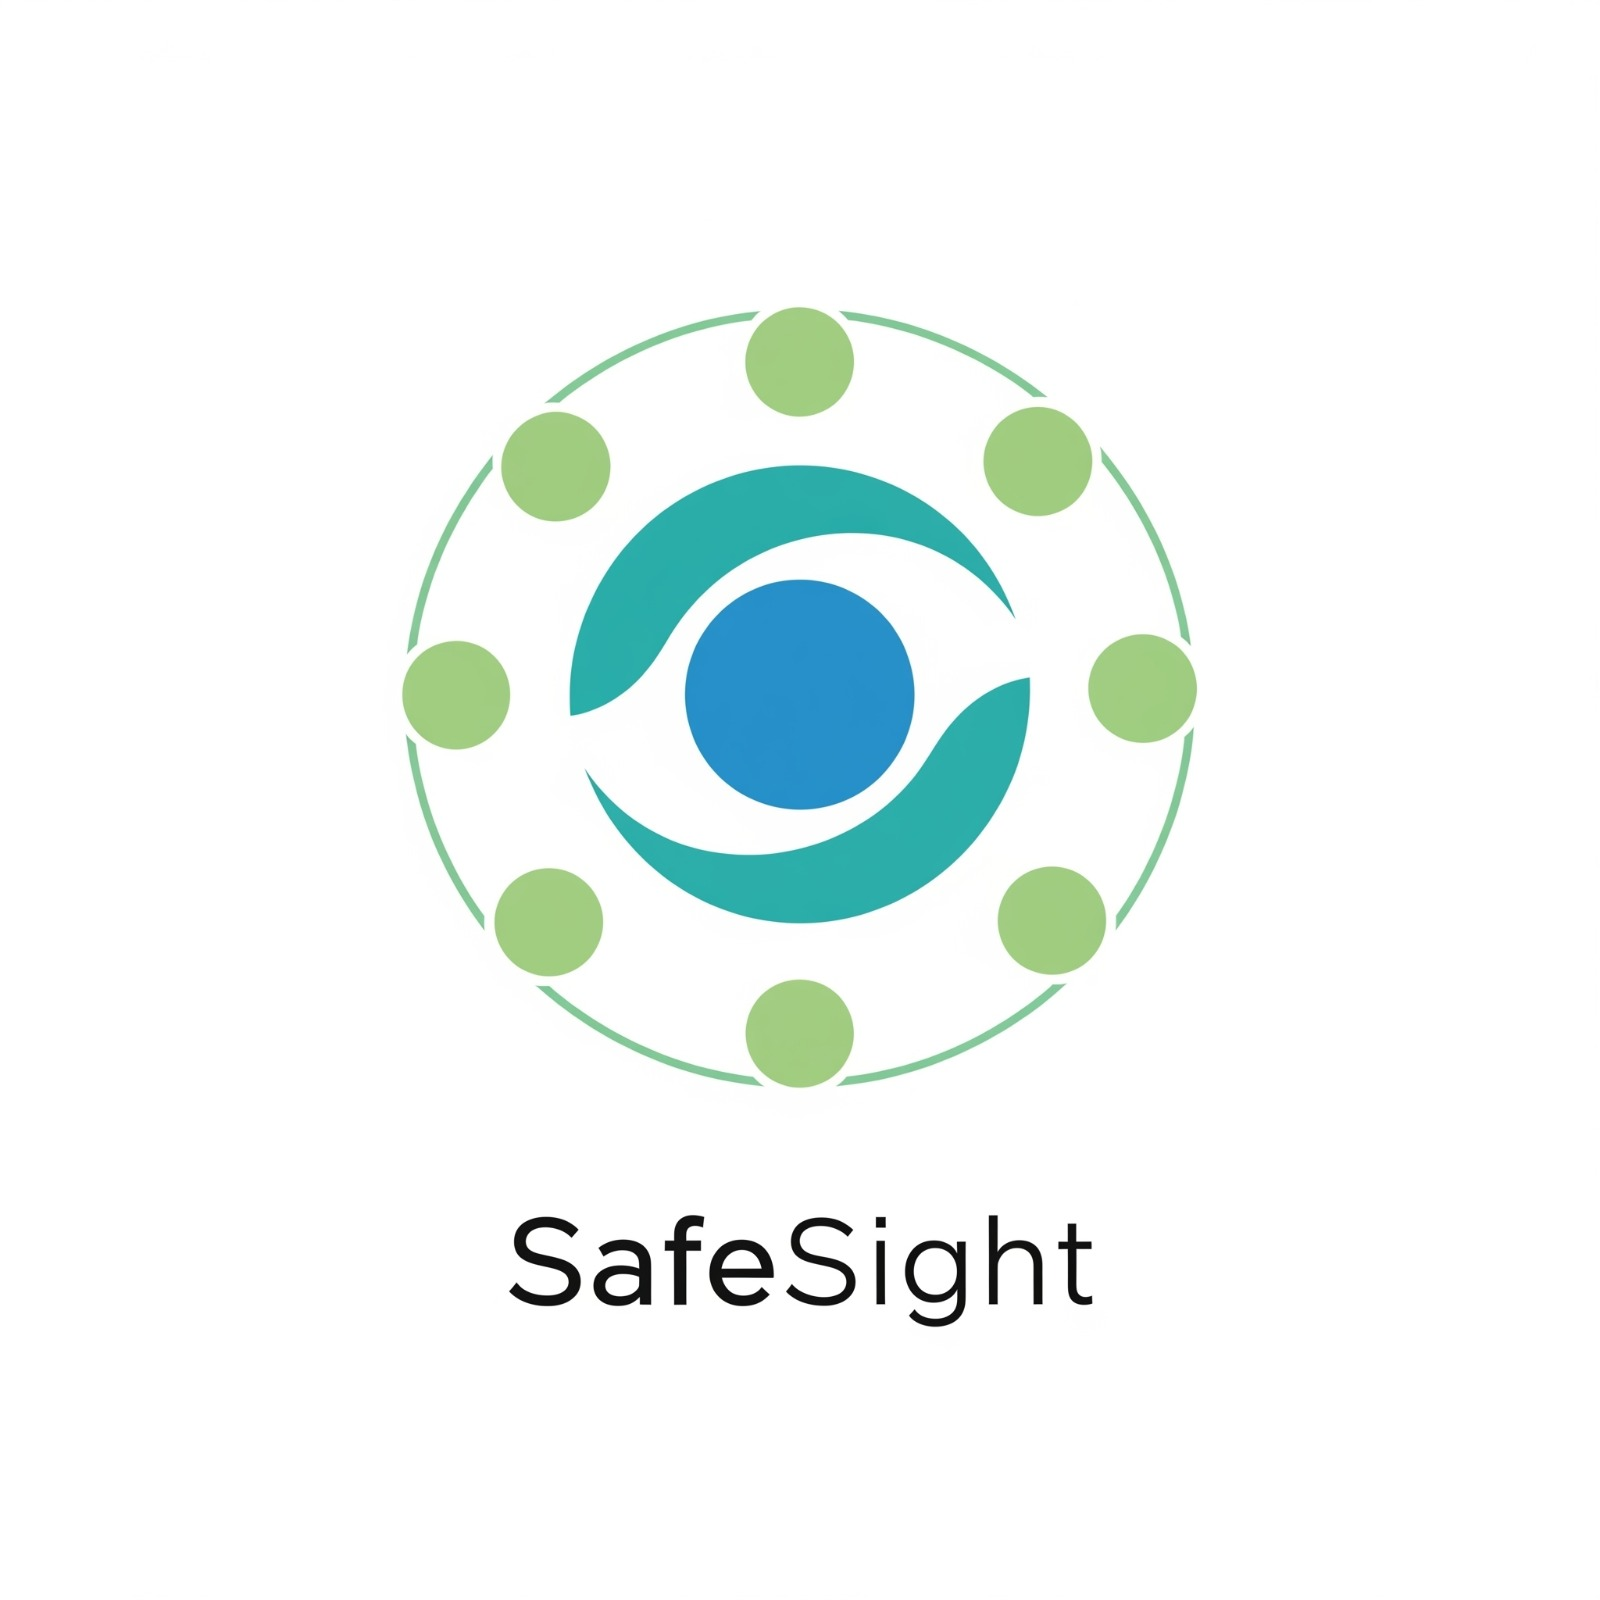
\includegraphics[width=0.3\textwidth]{./Media/Empresa.jpg}%
		}{%
			\fbox{\parbox{0.3\textwidth}{\centering Imagen ``Empresa.jpg'' no disponible}}%
		}
		\caption{Logotipo oficial del equipo desarrollador SafeSight.}\label{fig:logo_safesight}
\end{figure}

\subsection*{Justificación del Diseño}

El diseño fusiona seguridad y monitoreo avanzado.

\begin{itemize}
\item \textbf{Ojo central:} Representa visión, inteligencia y precisión.
\item \textbf{Red de nodos:} Simboliza protección integral de usuarios y datos.
\item \textbf{Círculo exterior:} Refuerza seguridad y control total.
\end{itemize}

	extit{Visión segura}: tecnología que vigila y protege el entorno.

\subsection*{Paleta de Colores}

Colores que transmiten profesionalismo y seguridad tecnológica.

\begin{itemize}
\item \textbf{Azul:} Confianza y estabilidad.
\item \textbf{Verde azulado:} Innovación y claridad.
\item \textbf{Verde claro:} Seguridad y positividad.
\end{itemize}

\subsection*{Tipografía}

Tipografía \textbf{sans-serif} moderna y geométrica, con CamelCase para destacar la unión de ``Safe'' y ``Sight''.

